\documentclass[1p]{elsarticle_modified}
%\bibliographystyle{elsarticle-num}

%\usepackage[colorlinks]{hyperref}
%\usepackage{abbrmath_seonhwa} %\Abb, \Ascr, \Acal ,\Abf, \Afrak
\usepackage{amsfonts}
\usepackage{amssymb}
\usepackage{amsmath}
\usepackage{amsthm}
\usepackage{scalefnt}
\usepackage{amsbsy}
\usepackage{kotex}
\usepackage{caption}
\usepackage{subfig}
\usepackage{color}
\usepackage{graphicx}
\usepackage{xcolor} %% white, black, red, green, blue, cyan, magenta, yellow
\usepackage{float}
\usepackage{setspace}
\usepackage{hyperref}

\usepackage{tikz}
\usetikzlibrary{arrows}

\usepackage{multirow}
\usepackage{array} % fixed length table
\usepackage{hhline}

%%%%%%%%%%%%%%%%%%%%%
\makeatletter
\renewcommand*\env@matrix[1][\arraystretch]{%
	\edef\arraystretch{#1}%
	\hskip -\arraycolsep
	\let\@ifnextchar\new@ifnextchar
	\array{*\c@MaxMatrixCols c}}
\makeatother %https://tex.stackexchange.com/questions/14071/how-can-i-increase-the-line-spacing-in-a-matrix
%%%%%%%%%%%%%%%

\usepackage[normalem]{ulem}

\newcommand{\msout}[1]{\ifmmode\text{\sout{\ensuremath{#1}}}\else\sout{#1}\fi}
%SOURCE: \msout is \stkout macro in https://tex.stackexchange.com/questions/20609/strikeout-in-math-mode

\newcommand{\cancel}[1]{
	\ifmmode
	{\color{red}\msout{#1}}
	\else
	{\color{red}\sout{#1}}
	\fi
}

\newcommand{\add}[1]{
	{\color{blue}\uwave{#1}}
}

\newcommand{\replace}[2]{
	\ifmmode
	{\color{red}\msout{#1}}{\color{blue}\uwave{#2}}
	\else
	{\color{red}\sout{#1}}{\color{blue}\uwave{#2}}
	\fi
}

\newcommand{\Sol}{\mathcal{S}} %segment
\newcommand{\D}{D} %diagram
\newcommand{\A}{\mathcal{A}} %arc


%%%%%%%%%%%%%%%%%%%%%%%%%%%%%5 test

\def\sl{\operatorname{\textup{SL}}(2,\Cbb)}
\def\psl{\operatorname{\textup{PSL}}(2,\Cbb)}
\def\quan{\mkern 1mu \triangleright \mkern 1mu}

\theoremstyle{definition}
\newtheorem{thm}{Theorem}[section]
\newtheorem{prop}[thm]{Proposition}
\newtheorem{lem}[thm]{Lemma}
\newtheorem{ques}[thm]{Question}
\newtheorem{cor}[thm]{Corollary}
\newtheorem{defn}[thm]{Definition}
\newtheorem{exam}[thm]{Example}
\newtheorem{rmk}[thm]{Remark}
\newtheorem{alg}[thm]{Algorithm}

\newcommand{\I}{\sqrt{-1}}
\begin{document}

%\begin{frontmatter}
%
%\title{Boundary parabolic representations of knots up to 8 crossings}
%
%%% Group authors per affiliation:
%\author{Yunhi Cho} 
%\address{Department of Mathematics, University of Seoul, Seoul, Korea}
%\ead{yhcho@uos.ac.kr}
%
%
%\author{Seonhwa Kim} %\fnref{s_kim}}
%\address{Center for Geometry and Physics, Institute for Basic Science, Pohang, 37673, Korea}
%\ead{ryeona17@ibs.re.kr}
%
%\author{Hyuk Kim}
%\address{Department of Mathematical Sciences, Seoul National University, Seoul 08826, Korea}
%\ead{hyukkim@snu.ac.kr}
%
%\author{Seokbeom Yoon}
%\address{Department of Mathematical Sciences, Seoul National University, Seoul, 08826,  Korea}
%\ead{sbyoon15@snu.ac.kr}
%
%\begin{abstract}
%We find all boundary parabolic representation of knots up to 8 crossings.
%
%\end{abstract}
%\begin{keyword}
%    \MSC[2010] 57M25 
%\end{keyword}
%
%\end{frontmatter}

%\linenumbers
%\tableofcontents
%
\newcommand\colored[1]{\textcolor{white}{\rule[-0.35ex]{0.8em}{1.4ex}}\kern-0.8em\color{red} #1}%
%\newcommand\colored[1]{\textcolor{white}{ #1}\kern-2.17ex	\textcolor{white}{ #1}\kern-1.81ex	\textcolor{white}{ #1}\kern-2.15ex\color{red}#1	}

{\Large $\underline{12a_{0570}~(K12a_{0570})}$}

\setlength{\tabcolsep}{10pt}
\renewcommand{\arraystretch}{1.6}
\vspace{1cm}\begin{tabular}{m{100pt}>{\centering\arraybackslash}m{274pt}}
\multirow{5}{120pt}{
	\centering
	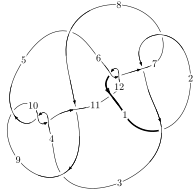
\includegraphics[width=112pt]{../../../GIT/diagram.site/Diagrams/png/1371_12a_0570.png}\\
\ \ \ A knot diagram\footnotemark}&
\allowdisplaybreaks
\textbf{Linearized knot diagam} \\
\cline{2-2}
 &
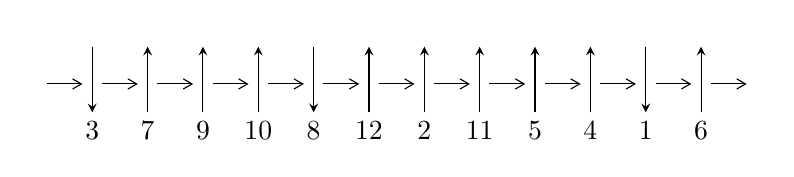
\begin{tikzpicture}[x=20pt, y=17pt]
	% nodes
	\node (C0) at (0, 0) {};
	\node (C1) at (1, 0) {};
	\node (C1U) at (1, +1) {};
	\node (C1D) at (1, -1) {3};

	\node (C2) at (2, 0) {};
	\node (C2U) at (2, +1) {};
	\node (C2D) at (2, -1) {7};

	\node (C3) at (3, 0) {};
	\node (C3U) at (3, +1) {};
	\node (C3D) at (3, -1) {9};

	\node (C4) at (4, 0) {};
	\node (C4U) at (4, +1) {};
	\node (C4D) at (4, -1) {10};

	\node (C5) at (5, 0) {};
	\node (C5U) at (5, +1) {};
	\node (C5D) at (5, -1) {8};

	\node (C6) at (6, 0) {};
	\node (C6U) at (6, +1) {};
	\node (C6D) at (6, -1) {12};

	\node (C7) at (7, 0) {};
	\node (C7U) at (7, +1) {};
	\node (C7D) at (7, -1) {2};

	\node (C8) at (8, 0) {};
	\node (C8U) at (8, +1) {};
	\node (C8D) at (8, -1) {11};

	\node (C9) at (9, 0) {};
	\node (C9U) at (9, +1) {};
	\node (C9D) at (9, -1) {5};

	\node (C10) at (10, 0) {};
	\node (C10U) at (10, +1) {};
	\node (C10D) at (10, -1) {4};

	\node (C11) at (11, 0) {};
	\node (C11U) at (11, +1) {};
	\node (C11D) at (11, -1) {1};

	\node (C12) at (12, 0) {};
	\node (C12U) at (12, +1) {};
	\node (C12D) at (12, -1) {6};
	\node (C13) at (13, 0) {};

	% arrows
	\draw[->,>={angle 60}]
	(C0) edge (C1) (C1) edge (C2) (C2) edge (C3) (C3) edge (C4) (C4) edge (C5) (C5) edge (C6) (C6) edge (C7) (C7) edge (C8) (C8) edge (C9) (C9) edge (C10) (C10) edge (C11) (C11) edge (C12) (C12) edge (C13) ;	\draw[->,>=stealth]
	(C1U) edge (C1D) (C2D) edge (C2U) (C3D) edge (C3U) (C4D) edge (C4U) (C5U) edge (C5D) (C6D) edge (C6U) (C7D) edge (C7U) (C8D) edge (C8U) (C9D) edge (C9U) (C10D) edge (C10U) (C11U) edge (C11D) (C12D) edge (C12U) ;
	\end{tikzpicture} \\
\hhline{~~} \\& 
\textbf{Solving Sequence} \\ \cline{2-2} 
 &
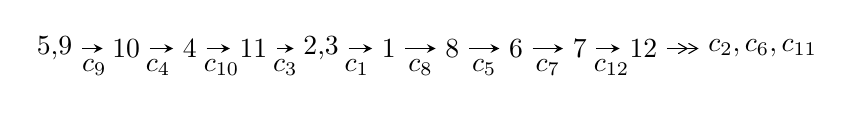
\begin{tikzpicture}[x=23pt, y=7pt]
	% node
	\node (A0) at (-1/8, 0) {5,9};
	\node (A1) at (1, 0) {10};
	\node (A2) at (2, 0) {4};
	\node (A3) at (3, 0) {11};
	\node (A4) at (65/16, 0) {2,3};
	\node (A5) at (41/8, 0) {1};
	\node (A6) at (49/8, 0) {8};
	\node (A7) at (57/8, 0) {6};
	\node (A8) at (65/8, 0) {7};
	\node (A9) at (73/8, 0) {12};
	\node (C1) at (1/2, -1) {$c_{9}$};
	\node (C2) at (3/2, -1) {$c_{4}$};
	\node (C3) at (5/2, -1) {$c_{10}$};
	\node (C4) at (7/2, -1) {$c_{3}$};
	\node (C5) at (37/8, -1) {$c_{1}$};
	\node (C6) at (45/8, -1) {$c_{8}$};
	\node (C7) at (53/8, -1) {$c_{5}$};
	\node (C8) at (61/8, -1) {$c_{7}$};
	\node (C9) at (69/8, -1) {$c_{12}$};
	\node (A10) at (11, 0) {$c_{2},c_{6},c_{11}$};

	% edge
	\draw[->,>=stealth]	
	(A0) edge (A1) (A1) edge (A2) (A2) edge (A3) (A3) edge (A4) (A4) edge (A5) (A5) edge (A6) (A6) edge (A7) (A7) edge (A8) (A8) edge (A9) ;
	\draw[->>,>={angle 60}]	
	(A9) edge (A10);
\end{tikzpicture} \\ 

\end{tabular} \\

\footnotetext{
The image of knot diagram is generated by the software ``\textbf{Draw programme}" developed by Andrew Bartholomew(\url{http://www.layer8.co.uk/maths/draw/index.htm\#Running-draw}), where we modified some parts for our purpose(\url{https://github.com/CATsTAILs/LinksPainter}).
}\phantom \\ \newline 
\centering \textbf{Ideals for irreducible components\footnotemark of $X_{\text{par}}$} 
 
\begin{align*}
I^u_{1}&=\langle 
u^{40}+3 u^{39}+\cdots+b+3,\;-3 u^{42}-9 u^{41}+\cdots+2 a-11,\;u^{43}+3 u^{42}+\cdots+11 u+2\rangle \\
I^u_{2}&=\langle 
190 u^{31} a+573 u^{31}+\cdots-125 a-709,\;- u^{31}-14 u^{29}+\cdots+a^2+a,\;u^{32}- u^{31}+\cdots-2 u+1\rangle \\
I^u_{3}&=\langle 
u^9+4 u^7+5 u^5- u^4+u^3-2 u^2+b,\;u^8+4 u^6+5 u^4+2 u^2+a+1,\;u^{10}+5 u^8+8 u^6+3 u^4- u^2+1\rangle \\
\\
\end{align*}
\raggedright * 3 irreducible components of $\dim_{\mathbb{C}}=0$, with total 117 representations.\\
\footnotetext{All coefficients of polynomials are rational numbers. But the coefficients are sometimes approximated in decimal forms when there is not enough margin.}
\newpage
\renewcommand{\arraystretch}{1}
\centering \section*{I. $I^u_{1}= \langle u^{40}+3 u^{39}+\cdots+b+3,\;-3 u^{42}-9 u^{41}+\cdots+2 a-11,\;u^{43}+3 u^{42}+\cdots+11 u+2 \rangle$}
\flushleft \textbf{(i) Arc colorings}\\
\begin{tabular}{m{7pt} m{180pt} m{7pt} m{180pt} }
\flushright $a_{5}=$&$\begin{pmatrix}0\\u\end{pmatrix}$ \\
\flushright $a_{9}=$&$\begin{pmatrix}1\\0\end{pmatrix}$ \\
\flushright $a_{10}=$&$\begin{pmatrix}1\\- u^2\end{pmatrix}$ \\
\flushright $a_{4}=$&$\begin{pmatrix}- u\\u^3+u\end{pmatrix}$ \\
\flushright $a_{11}=$&$\begin{pmatrix}u^2+1\\- u^4-2 u^2\end{pmatrix}$ \\
\flushright $a_{2}=$&$\begin{pmatrix}\frac{3}{2} u^{42}+\frac{9}{2} u^{41}+\cdots+23 u+\frac{11}{2}\\- u^{40}-3 u^{39}+\cdots-10 u-3\end{pmatrix}$ \\
\flushright $a_{3}=$&$\begin{pmatrix}- u^3-2 u\\u^3+u\end{pmatrix}$ \\
\flushright $a_{1}=$&$\begin{pmatrix}\frac{5}{2} u^{42}+\frac{15}{2} u^{41}+\cdots+41 u+\frac{19}{2}\\-2 u^{40}-5 u^{39}+\cdots-18 u-5\end{pmatrix}$ \\
\flushright $a_{8}=$&$\begin{pmatrix}- u^6-3 u^4-2 u^2+1\\u^8+4 u^6+4 u^4\end{pmatrix}$ \\
\flushright $a_{6}=$&$\begin{pmatrix}- u^{13}-6 u^{11}-13 u^9-10 u^7+2 u^5+4 u^3- u\\u^{15}+7 u^{13}+18 u^{11}+19 u^9+4 u^7-4 u^5+u\end{pmatrix}$ \\
\flushright $a_{7}=$&$\begin{pmatrix}\frac{1}{2} u^{42}+\frac{1}{2} u^{41}+\cdots+u+\frac{1}{2}\\u^{41}+2 u^{40}+\cdots+4 u+1\end{pmatrix}$ \\
\flushright $a_{12}=$&$\begin{pmatrix}-\frac{3}{2} u^{42}-\frac{9}{2} u^{41}+\cdots-25 u-\frac{9}{2}\\u^{40}+3 u^{39}+\cdots+11 u+3\end{pmatrix}$\\&\end{tabular}
\flushleft \textbf{(ii) Obstruction class $= -1$}\\~\\
\flushleft \textbf{(iii) Cusp Shapes $= 12 u^{42}+26 u^{41}+\cdots+114 u+38$}\\~\\
\newpage\renewcommand{\arraystretch}{1}
\flushleft \textbf{(iv) u-Polynomials at the component}\newline \\
\begin{tabular}{m{50pt}|m{274pt}}
Crossings & \hspace{64pt}u-Polynomials at each crossing \\
\hline $$\begin{aligned}c_{1},c_{11}\end{aligned}$$&$\begin{aligned}
&u^{43}+18 u^{42}+\cdots-5 u-1
\end{aligned}$\\
\hline $$\begin{aligned}c_{2},c_{6},c_{7}\\c_{12}\end{aligned}$$&$\begin{aligned}
&u^{43}+9 u^{41}+\cdots+u-1
\end{aligned}$\\
\hline $$\begin{aligned}c_{3}\end{aligned}$$&$\begin{aligned}
&u^{43}+3 u^{42}+\cdots+79 u-10
\end{aligned}$\\
\hline $$\begin{aligned}c_{4},c_{9},c_{10}\end{aligned}$$&$\begin{aligned}
&u^{43}-3 u^{42}+\cdots+11 u-2
\end{aligned}$\\
\hline $$\begin{aligned}c_{5}\end{aligned}$$&$\begin{aligned}
&u^{43}-21 u^{42}+\cdots+18607 u-1058
\end{aligned}$\\
\hline $$\begin{aligned}c_{8}\end{aligned}$$&$\begin{aligned}
&u^{43}+9 u^{42}+\cdots-863 u-88
\end{aligned}$\\
\hline
\end{tabular}\\~\\
\newpage\renewcommand{\arraystretch}{1}
\flushleft \textbf{(v) Riley Polynomials at the component}\newline \\
\begin{tabular}{m{50pt}|m{274pt}}
Crossings & \hspace{64pt}Riley Polynomials at each crossing \\
\hline $$\begin{aligned}c_{1},c_{11}\end{aligned}$$&$\begin{aligned}
&y^{43}+26 y^{42}+\cdots+67 y-1
\end{aligned}$\\
\hline $$\begin{aligned}c_{2},c_{6},c_{7}\\c_{12}\end{aligned}$$&$\begin{aligned}
&y^{43}+18 y^{42}+\cdots-5 y-1
\end{aligned}$\\
\hline $$\begin{aligned}c_{3}\end{aligned}$$&$\begin{aligned}
&y^{43}+3 y^{42}+\cdots+241 y-100
\end{aligned}$\\
\hline $$\begin{aligned}c_{4},c_{9},c_{10}\end{aligned}$$&$\begin{aligned}
&y^{43}+39 y^{42}+\cdots+17 y-4
\end{aligned}$\\
\hline $$\begin{aligned}c_{5}\end{aligned}$$&$\begin{aligned}
&y^{43}+3 y^{42}+\cdots+10766737 y-1119364
\end{aligned}$\\
\hline $$\begin{aligned}c_{8}\end{aligned}$$&$\begin{aligned}
&y^{43}+15 y^{42}+\cdots+108705 y-7744
\end{aligned}$\\
\hline
\end{tabular}\\~\\
\newpage\flushleft \textbf{(vi) Complex Volumes and Cusp Shapes}
$$\begin{array}{c|c|c}  
\text{Solutions to }I^u_{1}& \I (\text{vol} + \sqrt{-1}CS) & \text{Cusp shape}\\
 \hline 
\begin{aligned}
u &= \phantom{-}0.164014 + 0.946057 I \\
a &= \phantom{-}1.282900 - 0.345090 I \\
b &= \phantom{-}0.534324 - 0.151237 I\end{aligned}
 & \phantom{-}2.20216 - 1.04215 I & \phantom{-}8.70214 + 2.03700 I \\ \hline\begin{aligned}
u &= \phantom{-}0.164014 - 0.946057 I \\
a &= \phantom{-}1.282900 + 0.345090 I \\
b &= \phantom{-}0.534324 + 0.151237 I\end{aligned}
 & \phantom{-}2.20216 + 1.04215 I & \phantom{-}8.70214 - 2.03700 I \\ \hline\begin{aligned}
u &= \phantom{-}0.243062 + 1.100190 I \\
a &= -1.54071 - 0.64105 I \\
b &= -1.52314 + 0.64705 I\end{aligned}
 & -0.89825 + 9.73279 I & \phantom{-}4.53563 - 8.30440 I \\ \hline\begin{aligned}
u &= \phantom{-}0.243062 - 1.100190 I \\
a &= -1.54071 + 0.64105 I \\
b &= -1.52314 - 0.64705 I\end{aligned}
 & -0.89825 - 9.73279 I & \phantom{-}4.53563 + 8.30440 I \\ \hline\begin{aligned}
u &= -0.722534 + 0.301697 I \\
a &= \phantom{-}0.08578 + 3.01066 I \\
b &= -0.29124 - 2.70866 I\end{aligned}
 & -0.37610 - 13.45560 I & \phantom{-}5.29575 + 10.36544 I \\ \hline\begin{aligned}
u &= -0.722534 - 0.301697 I \\
a &= \phantom{-}0.08578 - 3.01066 I \\
b &= -0.29124 + 2.70866 I\end{aligned}
 & -0.37610 + 13.45560 I & \phantom{-}5.29575 - 10.36544 I \\ \hline\begin{aligned}
u &= -0.404425 + 0.657515 I \\
a &= -2.67151 + 0.36651 I \\
b &= \phantom{-}0.065501 - 1.014060 I\end{aligned}
 & -1.70851 + 9.45730 I & \phantom{-}2.82665 - 5.31681 I \\ \hline\begin{aligned}
u &= -0.404425 - 0.657515 I \\
a &= -2.67151 - 0.36651 I \\
b &= \phantom{-}0.065501 + 1.014060 I\end{aligned}
 & -1.70851 - 9.45730 I & \phantom{-}2.82665 + 5.31681 I \\ \hline\begin{aligned}
u &= -0.204544 + 0.730389 I \\
a &= \phantom{-}1.43841 - 0.73472 I \\
b &= \phantom{-}0.293207 + 0.580345 I\end{aligned}
 & \phantom{-}2.08121 - 1.04733 I & \phantom{-}8.22274 + 3.41589 I \\ \hline\begin{aligned}
u &= -0.204544 - 0.730389 I \\
a &= \phantom{-}1.43841 + 0.73472 I \\
b &= \phantom{-}0.293207 - 0.580345 I\end{aligned}
 & \phantom{-}2.08121 + 1.04733 I & \phantom{-}8.22274 - 3.41589 I\\
 \hline 
 \end{array}$$\newpage$$\begin{array}{c|c|c}  
\text{Solutions to }I^u_{1}& \I (\text{vol} + \sqrt{-1}CS) & \text{Cusp shape}\\
 \hline 
\begin{aligned}
u &= -0.644960 + 0.373766 I \\
a &= \phantom{-}0.760035 + 0.158019 I \\
b &= -1.138310 + 0.047746 I\end{aligned}
 & -3.38888 + 1.43692 I & \phantom{-}3.05929 - 2.01133 I \\ \hline\begin{aligned}
u &= -0.644960 - 0.373766 I \\
a &= \phantom{-}0.760035 - 0.158019 I \\
b &= -1.138310 - 0.047746 I\end{aligned}
 & -3.38888 - 1.43692 I & \phantom{-}3.05929 + 2.01133 I \\ \hline\begin{aligned}
u &= -0.703437 + 0.246639 I \\
a &= \phantom{-}0.66216 - 1.99434 I \\
b &= -0.29319 + 1.70932 I\end{aligned}
 & \phantom{-}3.84861 - 2.56258 I & \phantom{-}11.41433 + 1.98438 I \\ \hline\begin{aligned}
u &= -0.703437 - 0.246639 I \\
a &= \phantom{-}0.66216 + 1.99434 I \\
b &= -0.29319 - 1.70932 I\end{aligned}
 & \phantom{-}3.84861 + 2.56258 I & \phantom{-}11.41433 - 1.98438 I \\ \hline\begin{aligned}
u &= \phantom{-}0.702975 + 0.194251 I \\
a &= -0.86374 + 1.45652 I \\
b &= \phantom{-}0.330233 - 1.365890 I\end{aligned}
 & \phantom{-}4.46731 + 4.55873 I & \phantom{-}11.59252 - 6.90277 I \\ \hline\begin{aligned}
u &= \phantom{-}0.702975 - 0.194251 I \\
a &= -0.86374 - 1.45652 I \\
b &= \phantom{-}0.330233 + 1.365890 I\end{aligned}
 & \phantom{-}4.46731 - 4.55873 I & \phantom{-}11.59252 + 6.90277 I \\ \hline\begin{aligned}
u &= -0.522120 + 0.491654 I \\
a &= -0.240133 - 1.023150 I \\
b &= \phantom{-}0.500490 - 0.298029 I\end{aligned}
 & -3.88878 - 5.31369 I & \phantom{-}1.61265 + 8.28245 I \\ \hline\begin{aligned}
u &= -0.522120 - 0.491654 I \\
a &= -0.240133 + 1.023150 I \\
b &= \phantom{-}0.500490 + 0.298029 I\end{aligned}
 & -3.88878 + 5.31369 I & \phantom{-}1.61265 - 8.28245 I \\ \hline\begin{aligned}
u &= \phantom{-}0.704270 + 0.097056 I \\
a &= -0.35999 - 2.14445 I \\
b &= \phantom{-}0.72753 + 1.96810 I\end{aligned}
 & \phantom{-}2.11782 - 6.17915 I & \phantom{-}9.04327 + 4.42784 I \\ \hline\begin{aligned}
u &= \phantom{-}0.704270 - 0.097056 I \\
a &= -0.35999 + 2.14445 I \\
b &= \phantom{-}0.72753 - 1.96810 I\end{aligned}
 & \phantom{-}2.11782 + 6.17915 I & \phantom{-}9.04327 - 4.42784 I\\
 \hline 
 \end{array}$$\newpage$$\begin{array}{c|c|c}  
\text{Solutions to }I^u_{1}& \I (\text{vol} + \sqrt{-1}CS) & \text{Cusp shape}\\
 \hline 
\begin{aligned}
u &= \phantom{-}0.562309 + 0.373892 I \\
a &= -0.425293 - 0.567896 I \\
b &= \phantom{-}0.349891 + 0.140060 I\end{aligned}
 & -2.01863 + 1.75385 I & \phantom{-}5.78006 - 4.89342 I \\ \hline\begin{aligned}
u &= \phantom{-}0.562309 - 0.373892 I \\
a &= -0.425293 + 0.567896 I \\
b &= \phantom{-}0.349891 - 0.140060 I\end{aligned}
 & -2.01863 - 1.75385 I & \phantom{-}5.78006 + 4.89342 I \\ \hline\begin{aligned}
u &= \phantom{-}0.260662 + 1.303620 I \\
a &= \phantom{-}0.878955 + 0.346423 I \\
b &= \phantom{-}0.39384 - 2.51915 I\end{aligned}
 & -2.24110 - 2.69252 I & \phantom{-0.000000 } 0 \\ \hline\begin{aligned}
u &= \phantom{-}0.260662 - 1.303620 I \\
a &= \phantom{-}0.878955 - 0.346423 I \\
b &= \phantom{-}0.39384 + 2.51915 I\end{aligned}
 & -2.24110 + 2.69252 I & \phantom{-0.000000 } 0 \\ \hline\begin{aligned}
u &= -0.001427 + 1.338340 I \\
a &= -0.356373 - 0.037117 I \\
b &= \phantom{-}0.518324 - 0.887394 I\end{aligned}
 & -3.78341 - 1.46954 I & \phantom{-0.000000 } 0 \\ \hline\begin{aligned}
u &= -0.001427 - 1.338340 I \\
a &= -0.356373 + 0.037117 I \\
b &= \phantom{-}0.518324 + 0.887394 I\end{aligned}
 & -3.78341 + 1.46954 I & \phantom{-0.000000 } 0 \\ \hline\begin{aligned}
u &= -0.126955 + 1.361350 I \\
a &= -0.527328 - 0.405446 I \\
b &= \phantom{-}0.745333 - 0.463766 I\end{aligned}
 & -3.68931 - 1.78526 I & \phantom{-0.000000 } 0 \\ \hline\begin{aligned}
u &= -0.126955 - 1.361350 I \\
a &= -0.527328 + 0.405446 I \\
b &= \phantom{-}0.745333 + 0.463766 I\end{aligned}
 & -3.68931 + 1.78526 I & \phantom{-0.000000 } 0 \\ \hline\begin{aligned}
u &= \phantom{-}0.277378 + 1.369800 I \\
a &= -0.295618 - 0.850189 I \\
b &= -1.30294 + 1.86794 I\end{aligned}
 & -0.48560 + 8.11013 I & \phantom{-0.000000 } 0 \\ \hline\begin{aligned}
u &= \phantom{-}0.277378 - 1.369800 I \\
a &= -0.295618 + 0.850189 I \\
b &= -1.30294 - 1.86794 I\end{aligned}
 & -0.48560 - 8.11013 I & \phantom{-0.000000 } 0\\
 \hline 
 \end{array}$$\newpage$$\begin{array}{c|c|c}  
\text{Solutions to }I^u_{1}& \I (\text{vol} + \sqrt{-1}CS) & \text{Cusp shape}\\
 \hline 
\begin{aligned}
u &= -0.27745 + 1.39855 I \\
a &= -1.137110 + 0.389286 I \\
b &= -0.19324 - 2.23756 I\end{aligned}
 & -1.39190 - 6.12597 I & \phantom{-0.000000 } 0 \\ \hline\begin{aligned}
u &= -0.27745 - 1.39855 I \\
a &= -1.137110 - 0.389286 I \\
b &= -0.19324 + 2.23756 I\end{aligned}
 & -1.39190 + 6.12597 I & \phantom{-0.000000 } 0 \\ \hline\begin{aligned}
u &= \phantom{-}0.21669 + 1.43469 I \\
a &= \phantom{-}0.352241 + 0.027500 I \\
b &= -0.842082 - 0.581266 I\end{aligned}
 & -7.80581 + 4.63802 I & \phantom{-0.000000 } 0 \\ \hline\begin{aligned}
u &= \phantom{-}0.21669 - 1.43469 I \\
a &= \phantom{-}0.352241 - 0.027500 I \\
b &= -0.842082 + 0.581266 I\end{aligned}
 & -7.80581 - 4.63802 I & \phantom{-0.000000 } 0 \\ \hline\begin{aligned}
u &= -0.28325 + 1.42482 I \\
a &= \phantom{-}1.35303 - 1.05301 I \\
b &= \phantom{-}1.20627 + 3.61742 I\end{aligned}
 & -5.8954 - 17.1146 I & \phantom{-0.000000 } 0 \\ \hline\begin{aligned}
u &= -0.28325 - 1.42482 I \\
a &= \phantom{-}1.35303 + 1.05301 I \\
b &= \phantom{-}1.20627 - 3.61742 I\end{aligned}
 & -5.8954 + 17.1146 I & \phantom{-0.000000 } 0 \\ \hline\begin{aligned}
u &= -0.11220 + 1.45113 I \\
a &= \phantom{-}1.182720 + 0.686675 I \\
b &= -1.55004 - 0.11281 I\end{aligned}
 & -8.32121 + 7.81517 I & \phantom{-0.000000 } 0 \\ \hline\begin{aligned}
u &= -0.11220 - 1.45113 I \\
a &= \phantom{-}1.182720 - 0.686675 I \\
b &= -1.55004 + 0.11281 I\end{aligned}
 & -8.32121 - 7.81517 I & \phantom{-0.000000 } 0 \\ \hline\begin{aligned}
u &= -0.24228 + 1.44282 I \\
a &= -0.108809 - 0.420814 I \\
b &= \phantom{-}1.41781 - 0.62704 I\end{aligned}
 & -9.21691 - 1.80423 I & \phantom{-0.000000 } 0 \\ \hline\begin{aligned}
u &= -0.24228 - 1.44282 I \\
a &= -0.108809 + 0.420814 I \\
b &= \phantom{-}1.41781 + 0.62704 I\end{aligned}
 & -9.21691 + 1.80423 I & \phantom{-0.000000 } 0\\
 \hline 
 \end{array}$$\newpage$$\begin{array}{c|c|c}  
\text{Solutions to }I^u_{1}& \I (\text{vol} + \sqrt{-1}CS) & \text{Cusp shape}\\
 \hline 
\begin{aligned}
u &= -0.18017 + 1.45365 I \\
a &= -0.205904 + 0.631433 I \\
b &= \phantom{-}0.244371 + 0.099729 I\end{aligned}
 & -10.10500 - 7.84159 I & \phantom{-0.000000 } 0 \\ \hline\begin{aligned}
u &= -0.18017 - 1.45365 I \\
a &= -0.205904 - 0.631433 I \\
b &= \phantom{-}0.244371 - 0.099729 I\end{aligned}
 & -10.10500 + 7.84159 I & \phantom{-0.000000 } 0 \\ \hline\begin{aligned}
u &= -0.411211\phantom{ +0.000000I} \\
a &= \phantom{-}0.972593\phantom{ +0.000000I} \\
b &= -0.385880\phantom{ +0.000000I}\end{aligned}
 & \phantom{-}0.654283\phantom{ +0.000000I} & \phantom{-}15.3800\phantom{ +0.000000I}\\
 \hline 
 \end{array}$$\newpage\newpage\renewcommand{\arraystretch}{1}
\centering \section*{II. $I^u_{2}= \langle 190 u^{31} a+573 u^{31}+\cdots-125 a-709,\;- u^{31}-14 u^{29}+\cdots+a^2+a,\;u^{32}- u^{31}+\cdots-2 u+1 \rangle$}
\flushleft \textbf{(i) Arc colorings}\\
\begin{tabular}{m{7pt} m{180pt} m{7pt} m{180pt} }
\flushright $a_{5}=$&$\begin{pmatrix}0\\u\end{pmatrix}$ \\
\flushright $a_{9}=$&$\begin{pmatrix}1\\0\end{pmatrix}$ \\
\flushright $a_{10}=$&$\begin{pmatrix}1\\- u^2\end{pmatrix}$ \\
\flushright $a_{4}=$&$\begin{pmatrix}- u\\u^3+u\end{pmatrix}$ \\
\flushright $a_{11}=$&$\begin{pmatrix}u^2+1\\- u^4-2 u^2\end{pmatrix}$ \\
\flushright $a_{2}=$&$\begin{pmatrix}a\\-0.278592 a u^{31}-0.840176 u^{31}+\cdots+0.183284 a+1.03959\end{pmatrix}$ \\
\flushright $a_{3}=$&$\begin{pmatrix}- u^3-2 u\\u^3+u\end{pmatrix}$ \\
\flushright $a_{1}=$&$\begin{pmatrix}0.140762 a u^{31}-0.517595 u^{31}+\cdots+0.828446 a+0.458944\\-0.153959 a u^{31}-0.293255 u^{31}+\cdots+0.140762 a+0.482405\end{pmatrix}$ \\
\flushright $a_{8}=$&$\begin{pmatrix}- u^6-3 u^4-2 u^2+1\\u^8+4 u^6+4 u^4\end{pmatrix}$ \\
\flushright $a_{6}=$&$\begin{pmatrix}- u^{13}-6 u^{11}-13 u^9-10 u^7+2 u^5+4 u^3- u\\u^{15}+7 u^{13}+18 u^{11}+19 u^9+4 u^7-4 u^5+u\end{pmatrix}$ \\
\flushright $a_{7}=$&$\begin{pmatrix}0.293255 a u^{31}-1.03666 u^{31}+\cdots-0.482405 a+1.24780\\-0.214076 a u^{31}-0.0982405 u^{31}+\cdots-0.332845 a-0.895894\end{pmatrix}$ \\
\flushright $a_{12}=$&$\begin{pmatrix}0.0982405 a u^{31}-0.0747801 u^{31}+\cdots+0.895894 a+0.325513\\-0.0953079 a u^{31}-0.800587 u^{31}+\cdots-0.0557185 a+0.631965\end{pmatrix}$\\&\end{tabular}
\flushleft \textbf{(ii) Obstruction class $= -1$}\\~\\
\flushleft \textbf{(iii) Cusp Shapes $= -4 u^{31}+4 u^{30}-60 u^{29}+52 u^{28}-392 u^{27}+292 u^{26}-1448 u^{25}+908 u^{24}-3260 u^{23}+1640 u^{22}-4412 u^{21}+1548 u^{20}-3076 u^{19}+248 u^{18}-220 u^{17}-888 u^{16}+924 u^{15}-580 u^{14}-60 u^{13}+204 u^{12}-616 u^{11}+212 u^{10}-144 u^9-72 u^8+108 u^7-60 u^6+12 u^5+8 u^4-20 u^3+8 u^2-8 u+10$}\\~\\
\newpage\renewcommand{\arraystretch}{1}
\flushleft \textbf{(iv) u-Polynomials at the component}\newline \\
\begin{tabular}{m{50pt}|m{274pt}}
Crossings & \hspace{64pt}u-Polynomials at each crossing \\
\hline $$\begin{aligned}c_{1},c_{11}\end{aligned}$$&$\begin{aligned}
&u^{64}+35 u^{63}+\cdots+52 u^2+1
\end{aligned}$\\
\hline $$\begin{aligned}c_{2},c_{6},c_{7}\\c_{12}\end{aligned}$$&$\begin{aligned}
&u^{64}+u^{63}+\cdots+2 u+1
\end{aligned}$\\
\hline $$\begin{aligned}c_{3}\end{aligned}$$&$\begin{aligned}
&(u^{32}- u^{31}+\cdots+20 u^3+1)^{2}
\end{aligned}$\\
\hline $$\begin{aligned}c_{4},c_{9},c_{10}\end{aligned}$$&$\begin{aligned}
&(u^{32}+u^{31}+\cdots+2 u+1)^{2}
\end{aligned}$\\
\hline $$\begin{aligned}c_{5},c_{8}\end{aligned}$$&$\begin{aligned}
&(u^{32}+7 u^{31}+\cdots+104 u+17)^{2}
\end{aligned}$\\
\hline
\end{tabular}\\~\\
\newpage\renewcommand{\arraystretch}{1}
\flushleft \textbf{(v) Riley Polynomials at the component}\newline \\
\begin{tabular}{m{50pt}|m{274pt}}
Crossings & \hspace{64pt}Riley Polynomials at each crossing \\
\hline $$\begin{aligned}c_{1},c_{11}\end{aligned}$$&$\begin{aligned}
&y^{64}-13 y^{63}+\cdots+104 y+1
\end{aligned}$\\
\hline $$\begin{aligned}c_{2},c_{6},c_{7}\\c_{12}\end{aligned}$$&$\begin{aligned}
&y^{64}+35 y^{63}+\cdots+52 y^2+1
\end{aligned}$\\
\hline $$\begin{aligned}c_{3}\end{aligned}$$&$\begin{aligned}
&(y^{32}+y^{31}+\cdots+56 y^2+1)^{2}
\end{aligned}$\\
\hline $$\begin{aligned}c_{4},c_{9},c_{10}\end{aligned}$$&$\begin{aligned}
&(y^{32}+29 y^{31}+\cdots+4 y^2+1)^{2}
\end{aligned}$\\
\hline $$\begin{aligned}c_{5},c_{8}\end{aligned}$$&$\begin{aligned}
&(y^{32}+9 y^{31}+\cdots+3056 y+289)^{2}
\end{aligned}$\\
\hline
\end{tabular}\\~\\
\newpage\flushleft \textbf{(vi) Complex Volumes and Cusp Shapes}
$$\begin{array}{c|c|c}  
\text{Solutions to }I^u_{2}& \I (\text{vol} + \sqrt{-1}CS) & \text{Cusp shape}\\
 \hline 
\begin{aligned}
u &= -0.209460 + 1.051390 I \\
a &= -0.934884 - 0.232233 I \\
b &= -0.533239 - 0.058153 I\end{aligned}
 & \phantom{-}1.12671 - 4.25629 I & \phantom{-}7.47389 + 4.09777 I \\ \hline\begin{aligned}
u &= -0.209460 + 1.051390 I \\
a &= \phantom{-}1.55966 - 0.70578 I \\
b &= \phantom{-}1.32202 + 0.52410 I\end{aligned}
 & \phantom{-}1.12671 - 4.25629 I & \phantom{-}7.47389 + 4.09777 I \\ \hline\begin{aligned}
u &= -0.209460 - 1.051390 I \\
a &= -0.934884 + 0.232233 I \\
b &= -0.533239 + 0.058153 I\end{aligned}
 & \phantom{-}1.12671 + 4.25629 I & \phantom{-}7.47389 - 4.09777 I \\ \hline\begin{aligned}
u &= -0.209460 - 1.051390 I \\
a &= \phantom{-}1.55966 + 0.70578 I \\
b &= \phantom{-}1.32202 - 0.52410 I\end{aligned}
 & \phantom{-}1.12671 + 4.25629 I & \phantom{-}7.47389 - 4.09777 I \\ \hline\begin{aligned}
u &= \phantom{-}0.089089 + 1.108640 I \\
a &= \phantom{-}0.194552 - 0.198501 I \\
b &= \phantom{-}0.02787 - 1.84014 I\end{aligned}
 & -4.54650 + 1.65846 I & \phantom{-}3.56019 - 4.42001 I \\ \hline\begin{aligned}
u &= \phantom{-}0.089089 + 1.108640 I \\
a &= -1.76337 - 1.02559 I \\
b &= -1.54639 - 0.20893 I\end{aligned}
 & -4.54650 + 1.65846 I & \phantom{-}3.56019 - 4.42001 I \\ \hline\begin{aligned}
u &= \phantom{-}0.089089 - 1.108640 I \\
a &= \phantom{-}0.194552 + 0.198501 I \\
b &= \phantom{-}0.02787 + 1.84014 I\end{aligned}
 & -4.54650 - 1.65846 I & \phantom{-}3.56019 + 4.42001 I \\ \hline\begin{aligned}
u &= \phantom{-}0.089089 - 1.108640 I \\
a &= -1.76337 + 1.02559 I \\
b &= -1.54639 + 0.20893 I\end{aligned}
 & -4.54650 - 1.65846 I & \phantom{-}3.56019 + 4.42001 I \\ \hline\begin{aligned}
u &= \phantom{-}0.714631 + 0.281038 I \\
a &= -0.58887 - 1.89058 I \\
b &= \phantom{-}0.08278 + 1.63195 I\end{aligned}
 & \phantom{-}2.12380 + 7.91274 I & \phantom{-}8.55825 - 6.96002 I \\ \hline\begin{aligned}
u &= \phantom{-}0.714631 + 0.281038 I \\
a &= -0.44223 + 2.80524 I \\
b &= \phantom{-}0.42814 - 2.47045 I\end{aligned}
 & \phantom{-}2.12380 + 7.91274 I & \phantom{-}8.55825 - 6.96002 I\\
 \hline 
 \end{array}$$\newpage$$\begin{array}{c|c|c}  
\text{Solutions to }I^u_{2}& \I (\text{vol} + \sqrt{-1}CS) & \text{Cusp shape}\\
 \hline 
\begin{aligned}
u &= \phantom{-}0.714631 - 0.281038 I \\
a &= -0.58887 + 1.89058 I \\
b &= \phantom{-}0.08278 - 1.63195 I\end{aligned}
 & \phantom{-}2.12380 - 7.91274 I & \phantom{-}8.55825 + 6.96002 I \\ \hline\begin{aligned}
u &= \phantom{-}0.714631 - 0.281038 I \\
a &= -0.44223 - 2.80524 I \\
b &= \phantom{-}0.42814 + 2.47045 I\end{aligned}
 & \phantom{-}2.12380 - 7.91274 I & \phantom{-}8.55825 + 6.96002 I \\ \hline\begin{aligned}
u &= \phantom{-}0.339557 + 0.664733 I \\
a &= -1.37593 - 0.63879 I \\
b &= -0.035908 + 0.835219 I\end{aligned}
 & \phantom{-}0.65551 - 4.07051 I & \phantom{-}5.91410 + 1.89651 I \\ \hline\begin{aligned}
u &= \phantom{-}0.339557 + 0.664733 I \\
a &= \phantom{-}2.50163 - 0.00413 I \\
b &= -0.044254 - 0.702995 I\end{aligned}
 & \phantom{-}0.65551 - 4.07051 I & \phantom{-}5.91410 + 1.89651 I \\ \hline\begin{aligned}
u &= \phantom{-}0.339557 - 0.664733 I \\
a &= -1.37593 + 0.63879 I \\
b &= -0.035908 - 0.835219 I\end{aligned}
 & \phantom{-}0.65551 + 4.07051 I & \phantom{-}5.91410 - 1.89651 I \\ \hline\begin{aligned}
u &= \phantom{-}0.339557 - 0.664733 I \\
a &= \phantom{-}2.50163 + 0.00413 I \\
b &= -0.044254 + 0.702995 I\end{aligned}
 & \phantom{-}0.65551 + 4.07051 I & \phantom{-}5.91410 - 1.89651 I \\ \hline\begin{aligned}
u &= -0.672202 + 0.282270 I \\
a &= \phantom{-}0.506296 + 0.591013 I \\
b &= -1.271420 - 0.532717 I\end{aligned}
 & -3.28987 - 4.49550 I & \phantom{-}4.00000 + 7.21172 I \\ \hline\begin{aligned}
u &= -0.672202 + 0.282270 I \\
a &= \phantom{-}1.35780 + 3.33899 I \\
b &= -1.12075 - 2.55842 I\end{aligned}
 & -3.28987 - 4.49550 I & \phantom{-}4.00000 + 7.21172 I \\ \hline\begin{aligned}
u &= -0.672202 - 0.282270 I \\
a &= \phantom{-}0.506296 - 0.591013 I \\
b &= -1.271420 + 0.532717 I\end{aligned}
 & -3.28987 + 4.49550 I & \phantom{-}4.00000 - 7.21172 I \\ \hline\begin{aligned}
u &= -0.672202 - 0.282270 I \\
a &= \phantom{-}1.35780 - 3.33899 I \\
b &= -1.12075 + 2.55842 I\end{aligned}
 & -3.28987 + 4.49550 I & \phantom{-}4.00000 - 7.21172 I\\
 \hline 
 \end{array}$$\newpage$$\begin{array}{c|c|c}  
\text{Solutions to }I^u_{2}& \I (\text{vol} + \sqrt{-1}CS) & \text{Cusp shape}\\
 \hline 
\begin{aligned}
u &= -0.694439 + 0.142847 I \\
a &= \phantom{-}0.789254 + 0.891876 I \\
b &= -0.153418 - 0.883404 I\end{aligned}
 & \phantom{-}3.82740 + 0.78256 I & \phantom{-}11.62681 + 0.59259 I \\ \hline\begin{aligned}
u &= -0.694439 + 0.142847 I \\
a &= \phantom{-}0.47492 - 2.22804 I \\
b &= -0.62800 + 1.94416 I\end{aligned}
 & \phantom{-}3.82740 + 0.78256 I & \phantom{-}11.62681 + 0.59259 I \\ \hline\begin{aligned}
u &= -0.694439 - 0.142847 I \\
a &= \phantom{-}0.789254 - 0.891876 I \\
b &= -0.153418 + 0.883404 I\end{aligned}
 & \phantom{-}3.82740 - 0.78256 I & \phantom{-}11.62681 - 0.59259 I \\ \hline\begin{aligned}
u &= -0.694439 - 0.142847 I \\
a &= \phantom{-}0.47492 + 2.22804 I \\
b &= -0.62800 - 1.94416 I\end{aligned}
 & \phantom{-}3.82740 - 0.78256 I & \phantom{-}11.62681 - 0.59259 I \\ \hline\begin{aligned}
u &= \phantom{-}0.515560 + 0.370610 I \\
a &= -0.971553 - 0.576478 I \\
b &= \phantom{-}0.521901 + 0.456852 I\end{aligned}
 & -2.03323 + 1.65846 I & \phantom{-}4.43981 - 4.42001 I \\ \hline\begin{aligned}
u &= \phantom{-}0.515560 + 0.370610 I \\
a &= \phantom{-}0.092361 - 0.506624 I \\
b &= \phantom{-}0.160147 - 0.302293 I\end{aligned}
 & -2.03323 + 1.65846 I & \phantom{-}4.43981 - 4.42001 I \\ \hline\begin{aligned}
u &= \phantom{-}0.515560 - 0.370610 I \\
a &= -0.971553 + 0.576478 I \\
b &= \phantom{-}0.521901 - 0.456852 I\end{aligned}
 & -2.03323 - 1.65846 I & \phantom{-}4.43981 + 4.42001 I \\ \hline\begin{aligned}
u &= \phantom{-}0.515560 - 0.370610 I \\
a &= \phantom{-}0.092361 + 0.506624 I \\
b &= \phantom{-}0.160147 + 0.302293 I\end{aligned}
 & -2.03323 - 1.65846 I & \phantom{-}4.43981 + 4.42001 I \\ \hline\begin{aligned}
u &= \phantom{-}0.598306 + 0.209645 I \\
a &= \phantom{-}0.055218 + 0.713308 I \\
b &= \phantom{-}0.864572 - 0.880440 I\end{aligned}
 & -2.09042 + 1.01594 I & \phantom{-}7.95412 - 1.45531 I \\ \hline\begin{aligned}
u &= \phantom{-}0.598306 + 0.209645 I \\
a &= -1.36702 - 2.81720 I \\
b &= \phantom{-}1.01471 + 1.80896 I\end{aligned}
 & -2.09042 + 1.01594 I & \phantom{-}7.95412 - 1.45531 I\\
 \hline 
 \end{array}$$\newpage$$\begin{array}{c|c|c}  
\text{Solutions to }I^u_{2}& \I (\text{vol} + \sqrt{-1}CS) & \text{Cusp shape}\\
 \hline 
\begin{aligned}
u &= \phantom{-}0.598306 - 0.209645 I \\
a &= \phantom{-}0.055218 - 0.713308 I \\
b &= \phantom{-}0.864572 + 0.880440 I\end{aligned}
 & -2.09042 - 1.01594 I & \phantom{-}7.95412 + 1.45531 I \\ \hline\begin{aligned}
u &= \phantom{-}0.598306 - 0.209645 I \\
a &= -1.36702 + 2.81720 I \\
b &= \phantom{-}1.01471 - 1.80896 I\end{aligned}
 & -2.09042 - 1.01594 I & \phantom{-}7.95412 + 1.45531 I \\ \hline\begin{aligned}
u &= -0.265495 + 1.341380 I \\
a &= -1.020800 + 0.433430 I \\
b &= -0.36050 - 2.59349 I\end{aligned}
 & -0.84097 - 2.68301 I & \phantom{-}6.52130 + 2.36594 I \\ \hline\begin{aligned}
u &= -0.265495 + 1.341380 I \\
a &= \phantom{-}0.007855 - 0.645958 I \\
b &= \phantom{-}0.98543 + 1.23226 I\end{aligned}
 & -0.84097 - 2.68301 I & \phantom{-}6.52130 + 2.36594 I \\ \hline\begin{aligned}
u &= -0.265495 - 1.341380 I \\
a &= -1.020800 - 0.433430 I \\
b &= -0.36050 + 2.59349 I\end{aligned}
 & -0.84097 + 2.68301 I & \phantom{-}6.52130 - 2.36594 I \\ \hline\begin{aligned}
u &= -0.265495 - 1.341380 I \\
a &= \phantom{-}0.007855 + 0.645958 I \\
b &= \phantom{-}0.98543 - 1.23226 I\end{aligned}
 & -0.84097 + 2.68301 I & \phantom{-}6.52130 - 2.36594 I \\ \hline\begin{aligned}
u &= -0.323417 + 0.508294 I \\
a &= -0.520273 - 1.034610 I \\
b &= \phantom{-}0.287125 - 0.913296 I\end{aligned}
 & -4.48931 + 1.01594 I & \phantom{-}0.04588 - 1.45531 I \\ \hline\begin{aligned}
u &= -0.323417 + 0.508294 I \\
a &= -3.36072 - 0.80274 I \\
b &= \phantom{-}0.743295 - 0.386337 I\end{aligned}
 & -4.48931 + 1.01594 I & \phantom{-}0.04588 - 1.45531 I \\ \hline\begin{aligned}
u &= -0.323417 - 0.508294 I \\
a &= -0.520273 + 1.034610 I \\
b &= \phantom{-}0.287125 + 0.913296 I\end{aligned}
 & -4.48931 - 1.01594 I & \phantom{-}0.04588 + 1.45531 I \\ \hline\begin{aligned}
u &= -0.323417 - 0.508294 I \\
a &= -3.36072 + 0.80274 I \\
b &= \phantom{-}0.743295 + 0.386337 I\end{aligned}
 & -4.48931 - 1.01594 I & \phantom{-}0.04588 + 1.45531 I\\
 \hline 
 \end{array}$$\newpage$$\begin{array}{c|c|c}  
\text{Solutions to }I^u_{2}& \I (\text{vol} + \sqrt{-1}CS) & \text{Cusp shape}\\
 \hline 
\begin{aligned}
u &= \phantom{-}0.235723 + 1.392280 I \\
a &= \phantom{-}1.45838 + 0.35987 I \\
b &= -0.57974 - 2.88435 I\end{aligned}
 & -7.23525 + 4.07051 I & \phantom{-}2.08590 - 1.89651 I \\ \hline\begin{aligned}
u &= \phantom{-}0.235723 + 1.392280 I \\
a &= -0.320654 - 0.130453 I \\
b &= -1.43078 - 0.01572 I\end{aligned}
 & -7.23525 + 4.07051 I & \phantom{-}2.08590 - 1.89651 I \\ \hline\begin{aligned}
u &= \phantom{-}0.235723 - 1.392280 I \\
a &= \phantom{-}1.45838 - 0.35987 I \\
b &= -0.57974 + 2.88435 I\end{aligned}
 & -7.23525 - 4.07051 I & \phantom{-}2.08590 + 1.89651 I \\ \hline\begin{aligned}
u &= \phantom{-}0.235723 - 1.392280 I \\
a &= -0.320654 + 0.130453 I \\
b &= -1.43078 + 0.01572 I\end{aligned}
 & -7.23525 - 4.07051 I & \phantom{-}2.08590 + 1.89651 I \\ \hline\begin{aligned}
u &= -0.14428 + 1.41797 I \\
a &= \phantom{-}0.182119 + 0.762399 I \\
b &= \phantom{-}0.568805 + 0.605729 I\end{aligned}
 & -10.40710 - 0.78256 I & -3.62681 - 0.59259 I \\ \hline\begin{aligned}
u &= -0.14428 + 1.41797 I \\
a &= \phantom{-}0.86680 + 1.28541 I \\
b &= -2.41207 - 0.83594 I\end{aligned}
 & -10.40710 - 0.78256 I & -3.62681 - 0.59259 I \\ \hline\begin{aligned}
u &= -0.14428 - 1.41797 I \\
a &= \phantom{-}0.182119 - 0.762399 I \\
b &= \phantom{-}0.568805 - 0.605729 I\end{aligned}
 & -10.40710 + 0.78256 I & -3.62681 + 0.59259 I \\ \hline\begin{aligned}
u &= -0.14428 - 1.41797 I \\
a &= \phantom{-}0.86680 - 1.28541 I \\
b &= -2.41207 + 0.83594 I\end{aligned}
 & -10.40710 + 0.78256 I & -3.62681 + 0.59259 I \\ \hline\begin{aligned}
u &= \phantom{-}0.19271 + 1.41648 I \\
a &= \phantom{-}0.691663 - 0.425815 I \\
b &= -1.19278 - 0.82150 I\end{aligned}
 & -7.70645 + 4.25629 I & \phantom{-0.000000 } 0. - 4.09777 I \\ \hline\begin{aligned}
u &= \phantom{-}0.19271 + 1.41648 I \\
a &= -0.066784 + 0.334796 I \\
b &= -0.819907 + 0.086970 I\end{aligned}
 & -7.70645 + 4.25629 I & \phantom{-0.000000 } 0. - 4.09777 I\\
 \hline 
 \end{array}$$\newpage$$\begin{array}{c|c|c}  
\text{Solutions to }I^u_{2}& \I (\text{vol} + \sqrt{-1}CS) & \text{Cusp shape}\\
 \hline 
\begin{aligned}
u &= \phantom{-}0.19271 - 1.41648 I \\
a &= \phantom{-}0.691663 + 0.425815 I \\
b &= -1.19278 + 0.82150 I\end{aligned}
 & -7.70645 - 4.25629 I & \phantom{-0.000000 -}0. + 4.09777 I \\ \hline\begin{aligned}
u &= \phantom{-}0.19271 - 1.41648 I \\
a &= -0.066784 - 0.334796 I \\
b &= -0.819907 - 0.086970 I\end{aligned}
 & -7.70645 - 4.25629 I & \phantom{-0.000000 -}0. + 4.09777 I \\ \hline\begin{aligned}
u &= \phantom{-}0.10594 + 1.42756 I \\
a &= -0.918714 + 0.715280 I \\
b &= \phantom{-}1.54734 - 0.53710 I\end{aligned}
 & -5.73877 - 2.68301 I & \phantom{-}1.47870 + 2.36594 I \\ \hline\begin{aligned}
u &= \phantom{-}0.10594 + 1.42756 I \\
a &= \phantom{-}0.676636 - 0.372114 I \\
b &= -0.756124 - 0.741018 I\end{aligned}
 & -5.73877 - 2.68301 I & \phantom{-}1.47870 + 2.36594 I \\ \hline\begin{aligned}
u &= \phantom{-}0.10594 - 1.42756 I \\
a &= -0.918714 - 0.715280 I \\
b &= \phantom{-}1.54734 + 0.53710 I\end{aligned}
 & -5.73877 + 2.68301 I & \phantom{-}1.47870 - 2.36594 I \\ \hline\begin{aligned}
u &= \phantom{-}0.10594 - 1.42756 I \\
a &= \phantom{-}0.676636 + 0.372114 I \\
b &= -0.756124 + 0.741018 I\end{aligned}
 & -5.73877 + 2.68301 I & \phantom{-}1.47870 - 2.36594 I \\ \hline\begin{aligned}
u &= -0.26371 + 1.41237 I \\
a &= \phantom{-}0.230081 - 0.417931 I \\
b &= \phantom{-}1.66019 - 0.28514 I\end{aligned}
 & -8.70354 - 7.91274 I & \phantom{-0.000000 -}0. + 6.96002 I \\ \hline\begin{aligned}
u &= -0.26371 + 1.41237 I \\
a &= \phantom{-}1.02067 - 1.69275 I \\
b &= \phantom{-}2.33566 + 3.50017 I\end{aligned}
 & -8.70354 - 7.91274 I & \phantom{-0.000000 -}0. + 6.96002 I \\ \hline\begin{aligned}
u &= -0.26371 - 1.41237 I \\
a &= \phantom{-}0.230081 + 0.417931 I \\
b &= \phantom{-}1.66019 + 0.28514 I\end{aligned}
 & -8.70354 + 7.91274 I & \phantom{-0.000000 } 0. - 6.96002 I \\ \hline\begin{aligned}
u &= -0.26371 - 1.41237 I \\
a &= \phantom{-}1.02067 + 1.69275 I \\
b &= \phantom{-}2.33566 - 3.50017 I\end{aligned}
 & -8.70354 + 7.91274 I & \phantom{-0.000000 } 0. - 6.96002 I\\
 \hline 
 \end{array}$$\newpage$$\begin{array}{c|c|c}  
\text{Solutions to }I^u_{2}& \I (\text{vol} + \sqrt{-1}CS) & \text{Cusp shape}\\
 \hline 
\begin{aligned}
u &= \phantom{-}0.28148 + 1.41481 I \\
a &= \phantom{-}1.110910 + 0.401180 I \\
b &= \phantom{-}0.27105 - 2.03432 I\end{aligned}
 & -3.28987 + 11.53570 I & \phantom{-}4.00000 - 7.26982 I \\ \hline\begin{aligned}
u &= \phantom{-}0.28148 + 1.41481 I \\
a &= -1.12502 - 1.13544 I \\
b &= -1.43575 + 3.33825 I\end{aligned}
 & -3.28987 + 11.53570 I & \phantom{-}4.00000 - 7.26982 I \\ \hline\begin{aligned}
u &= \phantom{-}0.28148 - 1.41481 I \\
a &= \phantom{-}1.110910 - 0.401180 I \\
b &= \phantom{-}0.27105 + 2.03432 I\end{aligned}
 & -3.28987 - 11.53570 I & \phantom{-}4.00000 + 7.26982 I \\ \hline\begin{aligned}
u &= \phantom{-}0.28148 - 1.41481 I \\
a &= -1.12502 + 1.13544 I \\
b &= -1.43575 - 3.33825 I\end{aligned}
 & -3.28987 - 11.53570 I & \phantom{-}4.00000 + 7.26982 I\\
 \hline 
 \end{array}$$\newpage\newpage\renewcommand{\arraystretch}{1}
\centering \section*{III. $I^u_{3}= \langle u^9+4 u^7+5 u^5- u^4+u^3-2 u^2+b,\;u^8+4 u^6+5 u^4+2 u^2+a+1,\;u^{10}+5 u^8+8 u^6+3 u^4- u^2+1 \rangle$}
\flushleft \textbf{(i) Arc colorings}\\
\begin{tabular}{m{7pt} m{180pt} m{7pt} m{180pt} }
\flushright $a_{5}=$&$\begin{pmatrix}0\\u\end{pmatrix}$ \\
\flushright $a_{9}=$&$\begin{pmatrix}1\\0\end{pmatrix}$ \\
\flushright $a_{10}=$&$\begin{pmatrix}1\\- u^2\end{pmatrix}$ \\
\flushright $a_{4}=$&$\begin{pmatrix}- u\\u^3+u\end{pmatrix}$ \\
\flushright $a_{11}=$&$\begin{pmatrix}u^2+1\\- u^4-2 u^2\end{pmatrix}$ \\
\flushright $a_{2}=$&$\begin{pmatrix}- u^8-4 u^6-5 u^4-2 u^2-1\\- u^9-4 u^7-5 u^5+u^4- u^3+2 u^2\end{pmatrix}$ \\
\flushright $a_{3}=$&$\begin{pmatrix}- u^3-2 u\\u^3+u\end{pmatrix}$ \\
\flushright $a_{1}=$&$\begin{pmatrix}- u^8-4 u^6-5 u^4+u^3-2 u^2+2 u-1\\- u^9-4 u^7-5 u^5+u^4-2 u^3+2 u^2- u\end{pmatrix}$ \\
\flushright $a_{8}=$&$\begin{pmatrix}- u^6-3 u^4-2 u^2+1\\u^8+4 u^6+4 u^4\end{pmatrix}$ \\
\flushright $a_{6}=$&$\begin{pmatrix}u^7+4 u^5+4 u^3\\- u^7-3 u^5-2 u^3+u\end{pmatrix}$ \\
\flushright $a_{7}=$&$\begin{pmatrix}u^9+5 u^7- u^6+8 u^5-3 u^4+3 u^3-2 u^2- u+1\\- u^7-3 u^5-2 u^3+u-1\end{pmatrix}$ \\
\flushright $a_{12}=$&$\begin{pmatrix}- u^8-4 u^6-5 u^4+u^3- u^2+2 u\\- u^9-4 u^7-5 u^5-2 u^3- u\end{pmatrix}$\\&\end{tabular}
\flushleft \textbf{(ii) Obstruction class $= 1$}\\~\\
\flushleft \textbf{(iii) Cusp Shapes $= -4 u^6-12 u^4-8 u^2$}\\~\\
\newpage\renewcommand{\arraystretch}{1}
\flushleft \textbf{(iv) u-Polynomials at the component}\newline \\
\begin{tabular}{m{50pt}|m{274pt}}
Crossings & \hspace{64pt}u-Polynomials at each crossing \\
\hline $$\begin{aligned}c_{1},c_{11}\end{aligned}$$&$\begin{aligned}
&(u-1)^{10}
\end{aligned}$\\
\hline $$\begin{aligned}c_{2},c_{6},c_{7}\\c_{12}\end{aligned}$$&$\begin{aligned}
&(u^2+1)^5
\end{aligned}$\\
\hline $$\begin{aligned}c_{3}\end{aligned}$$&$\begin{aligned}
&u^{10}+u^8+8 u^6+3 u^4+3 u^2+1
\end{aligned}$\\
\hline $$\begin{aligned}c_{4},c_{9},c_{10}\end{aligned}$$&$\begin{aligned}
&u^{10}+5 u^8+8 u^6+3 u^4- u^2+1
\end{aligned}$\\
\hline $$\begin{aligned}c_{5}\end{aligned}$$&$\begin{aligned}
&u^{10}-3 u^8+4 u^6- u^4- u^2+1
\end{aligned}$\\
\hline $$\begin{aligned}c_{8}\end{aligned}$$&$\begin{aligned}
&(u^5- u^4+2 u^3- u^2+u-1)^2
\end{aligned}$\\
\hline
\end{tabular}\\~\\
\newpage\renewcommand{\arraystretch}{1}
\flushleft \textbf{(v) Riley Polynomials at the component}\newline \\
\begin{tabular}{m{50pt}|m{274pt}}
Crossings & \hspace{64pt}Riley Polynomials at each crossing \\
\hline $$\begin{aligned}c_{1},c_{11}\end{aligned}$$&$\begin{aligned}
&(y-1)^{10}
\end{aligned}$\\
\hline $$\begin{aligned}c_{2},c_{6},c_{7}\\c_{12}\end{aligned}$$&$\begin{aligned}
&(y+1)^{10}
\end{aligned}$\\
\hline $$\begin{aligned}c_{3}\end{aligned}$$&$\begin{aligned}
&(y^5+y^4+8 y^3+3 y^2+3 y+1)^2
\end{aligned}$\\
\hline $$\begin{aligned}c_{4},c_{9},c_{10}\end{aligned}$$&$\begin{aligned}
&(y^5+5 y^4+8 y^3+3 y^2- y+1)^2
\end{aligned}$\\
\hline $$\begin{aligned}c_{5}\end{aligned}$$&$\begin{aligned}
&(y^5-3 y^4+4 y^3- y^2- y+1)^2
\end{aligned}$\\
\hline $$\begin{aligned}c_{8}\end{aligned}$$&$\begin{aligned}
&(y^5+3 y^4+4 y^3+y^2- y-1)^2
\end{aligned}$\\
\hline
\end{tabular}\\~\\
\newpage\flushleft \textbf{(vi) Complex Volumes and Cusp Shapes}
$$\begin{array}{c|c|c}  
\text{Solutions to }I^u_{3}& \I (\text{vol} + \sqrt{-1}CS) & \text{Cusp shape}\\
 \hline 
\begin{aligned}
u &= \phantom{-0.000000 -}1.217740 I \\
a &= -0.821196\phantom{ +0.000000I} \\
b &= -0.76683 - 1.58802 I\end{aligned}
 & -5.69095\phantom{ +0.000000I} & -1.48110\phantom{ +0.000000I} \\ \hline\begin{aligned}
u &= \phantom{-0.000000 } -1.217740 I \\
a &= -0.821196\phantom{ +0.000000I} \\
b &= -0.76683 + 1.58802 I\end{aligned}
 & -5.69095\phantom{ +0.000000I} & -1.48110\phantom{ +0.000000I} \\ \hline\begin{aligned}
u &= \phantom{-}0.549911 + 0.309916 I \\
a &= -0.77780 - 1.38013 I \\
b &= \phantom{-}0.896862 + 0.383681 I\end{aligned}
 & -3.61897 + 1.53058 I & -0.51511 - 4.43065 I \\ \hline\begin{aligned}
u &= \phantom{-}0.549911 - 0.309916 I \\
a &= -0.77780 + 1.38013 I \\
b &= \phantom{-}0.896862 - 0.383681 I\end{aligned}
 & -3.61897 - 1.53058 I & -0.51511 + 4.43065 I \\ \hline\begin{aligned}
u &= -0.549911 + 0.309916 I \\
a &= -0.77780 + 1.38013 I \\
b &= -0.218641 - 1.261070 I\end{aligned}
 & -3.61897 - 1.53058 I & -0.51511 + 4.43065 I \\ \hline\begin{aligned}
u &= -0.549911 - 0.309916 I \\
a &= -0.77780 - 1.38013 I \\
b &= -0.218641 + 1.261070 I\end{aligned}
 & -3.61897 + 1.53058 I & -0.51511 - 4.43065 I \\ \hline\begin{aligned}
u &= -0.21917 + 1.41878 I \\
a &= \phantom{-}0.688402 - 0.106340 I \\
b &= \phantom{-}0.638115 + 0.967447 I\end{aligned}
 & -9.16243 - 4.40083 I & -4.74431 + 3.49859 I \\ \hline\begin{aligned}
u &= -0.21917 - 1.41878 I \\
a &= \phantom{-}0.688402 + 0.106340 I \\
b &= \phantom{-}0.638115 - 0.967447 I\end{aligned}
 & -9.16243 + 4.40083 I & -4.74431 - 3.49859 I \\ \hline\begin{aligned}
u &= \phantom{-}0.21917 + 1.41878 I \\
a &= \phantom{-}0.688402 + 0.106340 I \\
b &= -1.54951 - 1.43286 I\end{aligned}
 & -9.16243 + 4.40083 I & -4.74431 - 3.49859 I \\ \hline\begin{aligned}
u &= \phantom{-}0.21917 - 1.41878 I \\
a &= \phantom{-}0.688402 - 0.106340 I \\
b &= -1.54951 + 1.43286 I\end{aligned}
 & -9.16243 - 4.40083 I & -4.74431 + 3.49859 I\\
 \hline 
 \end{array}$$\newpage
\newpage\renewcommand{\arraystretch}{1}
\centering \section*{ IV. u-Polynomials}
\begin{tabular}{m{50pt}|m{274pt}}
Crossings & \hspace{64pt}u-Polynomials at each crossing \\
\hline $$\begin{aligned}c_{1},c_{11}\end{aligned}$$&$\begin{aligned}
&((u-1)^{10})(u^{43}+18 u^{42}+\cdots-5 u-1)(u^{64}+35 u^{63}+\cdots+52 u^2+1)
\end{aligned}$\\
\hline $$\begin{aligned}c_{2},c_{6},c_{7}\\c_{12}\end{aligned}$$&$\begin{aligned}
&((u^2+1)^5)(u^{43}+9 u^{41}+\cdots+u-1)(u^{64}+u^{63}+\cdots+2 u+1)
\end{aligned}$\\
\hline $$\begin{aligned}c_{3}\end{aligned}$$&$\begin{aligned}
&(u^{10}+u^8+8 u^6+3 u^4+3 u^2+1)(u^{32}- u^{31}+\cdots+20 u^3+1)^{2}\\
&\cdot(u^{43}+3 u^{42}+\cdots+79 u-10)
\end{aligned}$\\
\hline $$\begin{aligned}c_{4},c_{9},c_{10}\end{aligned}$$&$\begin{aligned}
&(u^{10}+5 u^8+8 u^6+3 u^4- u^2+1)(u^{32}+u^{31}+\cdots+2 u+1)^{2}\\
&\cdot(u^{43}-3 u^{42}+\cdots+11 u-2)
\end{aligned}$\\
\hline $$\begin{aligned}c_{5}\end{aligned}$$&$\begin{aligned}
&(u^{10}-3 u^8+4 u^6- u^4- u^2+1)(u^{32}+7 u^{31}+\cdots+104 u+17)^{2}\\
&\cdot(u^{43}-21 u^{42}+\cdots+18607 u-1058)
\end{aligned}$\\
\hline $$\begin{aligned}c_{8}\end{aligned}$$&$\begin{aligned}
&((u^5- u^4+2 u^3- u^2+u-1)^2)(u^{32}+7 u^{31}+\cdots+104 u+17)^{2}\\
&\cdot(u^{43}+9 u^{42}+\cdots-863 u-88)
\end{aligned}$\\
\hline
\end{tabular}\newpage\renewcommand{\arraystretch}{1}
\centering \section*{ V. Riley Polynomials}
\begin{tabular}{m{50pt}|m{274pt}}
Crossings & \hspace{64pt}Riley Polynomials at each crossing \\
\hline $$\begin{aligned}c_{1},c_{11}\end{aligned}$$&$\begin{aligned}
&((y-1)^{10})(y^{43}+26 y^{42}+\cdots+67 y-1)(y^{64}-13 y^{63}+\cdots+104 y+1)
\end{aligned}$\\
\hline $$\begin{aligned}c_{2},c_{6},c_{7}\\c_{12}\end{aligned}$$&$\begin{aligned}
&((y+1)^{10})(y^{43}+18 y^{42}+\cdots-5 y-1)(y^{64}+35 y^{63}+\cdots+52 y^2+1)
\end{aligned}$\\
\hline $$\begin{aligned}c_{3}\end{aligned}$$&$\begin{aligned}
&((y^5+y^4+8 y^3+3 y^2+3 y+1)^2)(y^{32}+y^{31}+\cdots+56 y^2+1)^{2}\\
&\cdot(y^{43}+3 y^{42}+\cdots+241 y-100)
\end{aligned}$\\
\hline $$\begin{aligned}c_{4},c_{9},c_{10}\end{aligned}$$&$\begin{aligned}
&((y^5+5 y^4+8 y^3+3 y^2- y+1)^2)(y^{32}+29 y^{31}+\cdots+4 y^2+1)^{2}\\
&\cdot(y^{43}+39 y^{42}+\cdots+17 y-4)
\end{aligned}$\\
\hline $$\begin{aligned}c_{5}\end{aligned}$$&$\begin{aligned}
&((y^5-3 y^4+4 y^3- y^2- y+1)^2)(y^{32}+9 y^{31}+\cdots+3056 y+289)^{2}\\
&\cdot(y^{43}+3 y^{42}+\cdots+10766737 y-1119364)
\end{aligned}$\\
\hline $$\begin{aligned}c_{8}\end{aligned}$$&$\begin{aligned}
&((y^5+3 y^4+4 y^3+y^2- y-1)^2)(y^{32}+9 y^{31}+\cdots+3056 y+289)^{2}\\
&\cdot(y^{43}+15 y^{42}+\cdots+108705 y-7744)
\end{aligned}$\\
\hline
\end{tabular}
\vskip 2pc
\end{document}